\documentclass[tikz,border=5pt]{standalone}

\usepackage{tikz}
\usetikzlibrary{arrows.meta,positioning,calc}

\begin{document}
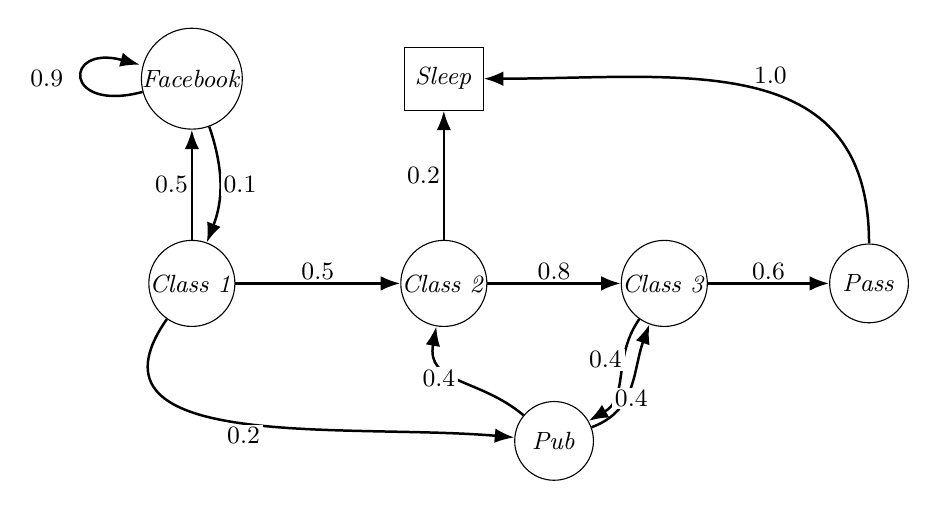
\begin{tikzpicture}[
  >=Latex,
  every node/.style={font=\small},
  state/.style={circle, draw, minimum size=10mm, inner sep=0pt},
  term/.style={rectangle, draw, minimum width=10mm, minimum height=8mm, inner sep=2pt},
  edge/.style={->, line width=0.9pt},
  lab/.style={midway, fill=white, inner sep=1pt}
]

% --- nodes (absolute placement for fidelity) ---
\node[state] (fb)    at (0,4) {\textit{Facebook}};
\node[state] (c1)    at (0,1.4) {\textit{Class 1}};
\node[state] (c2)    at (3.2,1.4) {\textit{Class 2}};
\node[state] (c3)    at (6.0,1.4) {\textit{Class 3}};
\node[state] (pass)  at (8.6,1.4) {\textit{Pass}};
\node[state] (pub)   at (4.6,-0.6) {\textit{Pub}};
\node[term]  (sleep) at (3.2,4) {\textit{Sleep}};

% --- edges ---
% Facebook self-loop and to Class 1
\draw[edge] (fb) edge[loop left] node[lab, xshift=-2mm] {0.9} (fb);
\draw[edge] (fb) to[bend left=20] node[lab, right] {0.1} (c1);

% Class 1 to Facebook and to Class 2
\draw[edge] (c1) -- node[lab, left] {0.5} (fb);
\draw[edge] (c1) -- node[lab, above] {0.5} (c2);

% Class 2 to Sleep and to Class 3
\draw[edge] (c2) -- node[lab, left] {0.2} (sleep);
\draw[edge] (c2) -- node[lab, above] {0.8} (c3);

% Class 3 to Pass
\draw[edge] (c3) -- node[lab, above] {0.6} (pass);

% Pass to Sleep (large curved)
\draw[edge] (pass) to[out=90, in=0, looseness=1.2] node[lab, above right] {1.0} (sleep);

% Lower transitions (via Pub)
\draw[edge] (c1) to[out=235, in=175, looseness=1.15] node[lab, below] {0.2} (pub);
\draw[edge] (c3) to[out=235, in=30, looseness=1.05] node[lab, near start, below left] {0.4} (pub);
\draw[edge] (pub) to[out=140, in=260, looseness=1.2] node[lab, left] {0.4} (c2);
\draw[edge] (pub) to[out=20, in=250, looseness=1.05] node[lab, below] {0.4} (c3);

\end{tikzpicture}
\end{document}
